% Created 2022-05-23 Mon 10:20
% Intended LaTeX compiler: xelatex
\documentclass[letterpaper]{article}
\usepackage{graphicx}
\usepackage{longtable}
\usepackage{wrapfig}
\usepackage{rotating}
\usepackage[normalem]{ulem}
\usepackage{amsmath}
\usepackage{amssymb}
\usepackage{capt-of}
\usepackage{hyperref}
\usepackage[margin=1in]{geometry}
\setlength{\parindent}{0pt}
\usepackage[margin=1in]{geometry}
\usepackage{fontspec}
\usepackage{svg}
\usepackage{tikz}
\usepackage{cancel}
\usepackage{pgfplots}
\usepackage{indentfirst}
\setmainfont[ItalicFont = HelveticaNeue-Italic, BoldFont = HelveticaNeue-Bold, BoldItalicFont = HelveticaNeue-BoldItalic]{HelveticaNeue}
\newfontfamily\NHLight[ItalicFont = HelveticaNeue-LightItalic, BoldFont       = HelveticaNeue-UltraLight, BoldItalicFont = HelveticaNeue-UltraLightItalic]{HelveticaNeue-Light}
\newcommand\textrmlf[1]{{\NHLight#1}}
\newcommand\textitlf[1]{{\NHLight\itshape#1}}
\let\textbflf\textrm
\newcommand\textulf[1]{{\NHLight\bfseries#1}}
\newcommand\textuitlf[1]{{\NHLight\bfseries\itshape#1}}
\usepackage{fancyhdr}
\usepackage{csquotes}
\pagestyle{fancy}
\usepackage{titlesec}
\usepackage{titling}
\makeatletter
\lhead{\textbf{\@title}}
\makeatother
\rhead{\textrmlf{Written} \today}
\lfoot{\theauthor\ \textbullet \ \textbf{2021-2022}}
\cfoot{}
\rfoot{\textrmlf{Page} \thepage}
\renewcommand{\tableofcontents}{}
\titleformat{\section} {\Large} {\textrmlf{\thesection} {|}} {0.3em} {\textbf}
\titleformat{\subsection} {\large} {\textrmlf{\thesubsection} {|}} {0.2em} {\textbf}
\titleformat{\subsubsection} {\large} {\textrmlf{\thesubsubsection} {|}} {0.1em} {\textbf}
\setlength{\parskip}{0.45em}
\renewcommand\maketitle{}
\author{Houjun Liu}
\date{\today}
\title{MVC 2 PS\#29}
\hypersetup{
 pdfauthor={Houjun Liu},
 pdftitle={MVC 2 PS\#29},
 pdfkeywords={},
 pdfsubject={},
 pdfcreator={Emacs 28.0.91 (Org mode 9.5.2)}, 
 pdflang={English}}
\begin{document}

\maketitle
\tableofcontents


\section{A surface integral}
\label{sec:org0b433ae}
We are defining a function:

\begin{equation}
   f(x,y,z) = y^2 
\end{equation}

and slicing out a vertical organ pipe shape with a sliced edge. That is:

\begin{equation}
   x^2 + z^2 = 1 
\end{equation}

bounded by \(y>0\) and \(y<3-x\).

Let's plot this:

\begin{verbatim}
var('x,y,z')
f = y^2

implicit_plot3d(x^2+z^2 == 1, (x,-1,1), (y,0,4), (z, -1,1), region=(lambda x,y,z: y>0 and y<3-x), color=(f,colormaps.cool), plot_points=100)
\end{verbatim}

\begin{verbatim}
(x, y, z)
Launched html viewer for Graphics3d Object
\end{verbatim}


\begin{center}
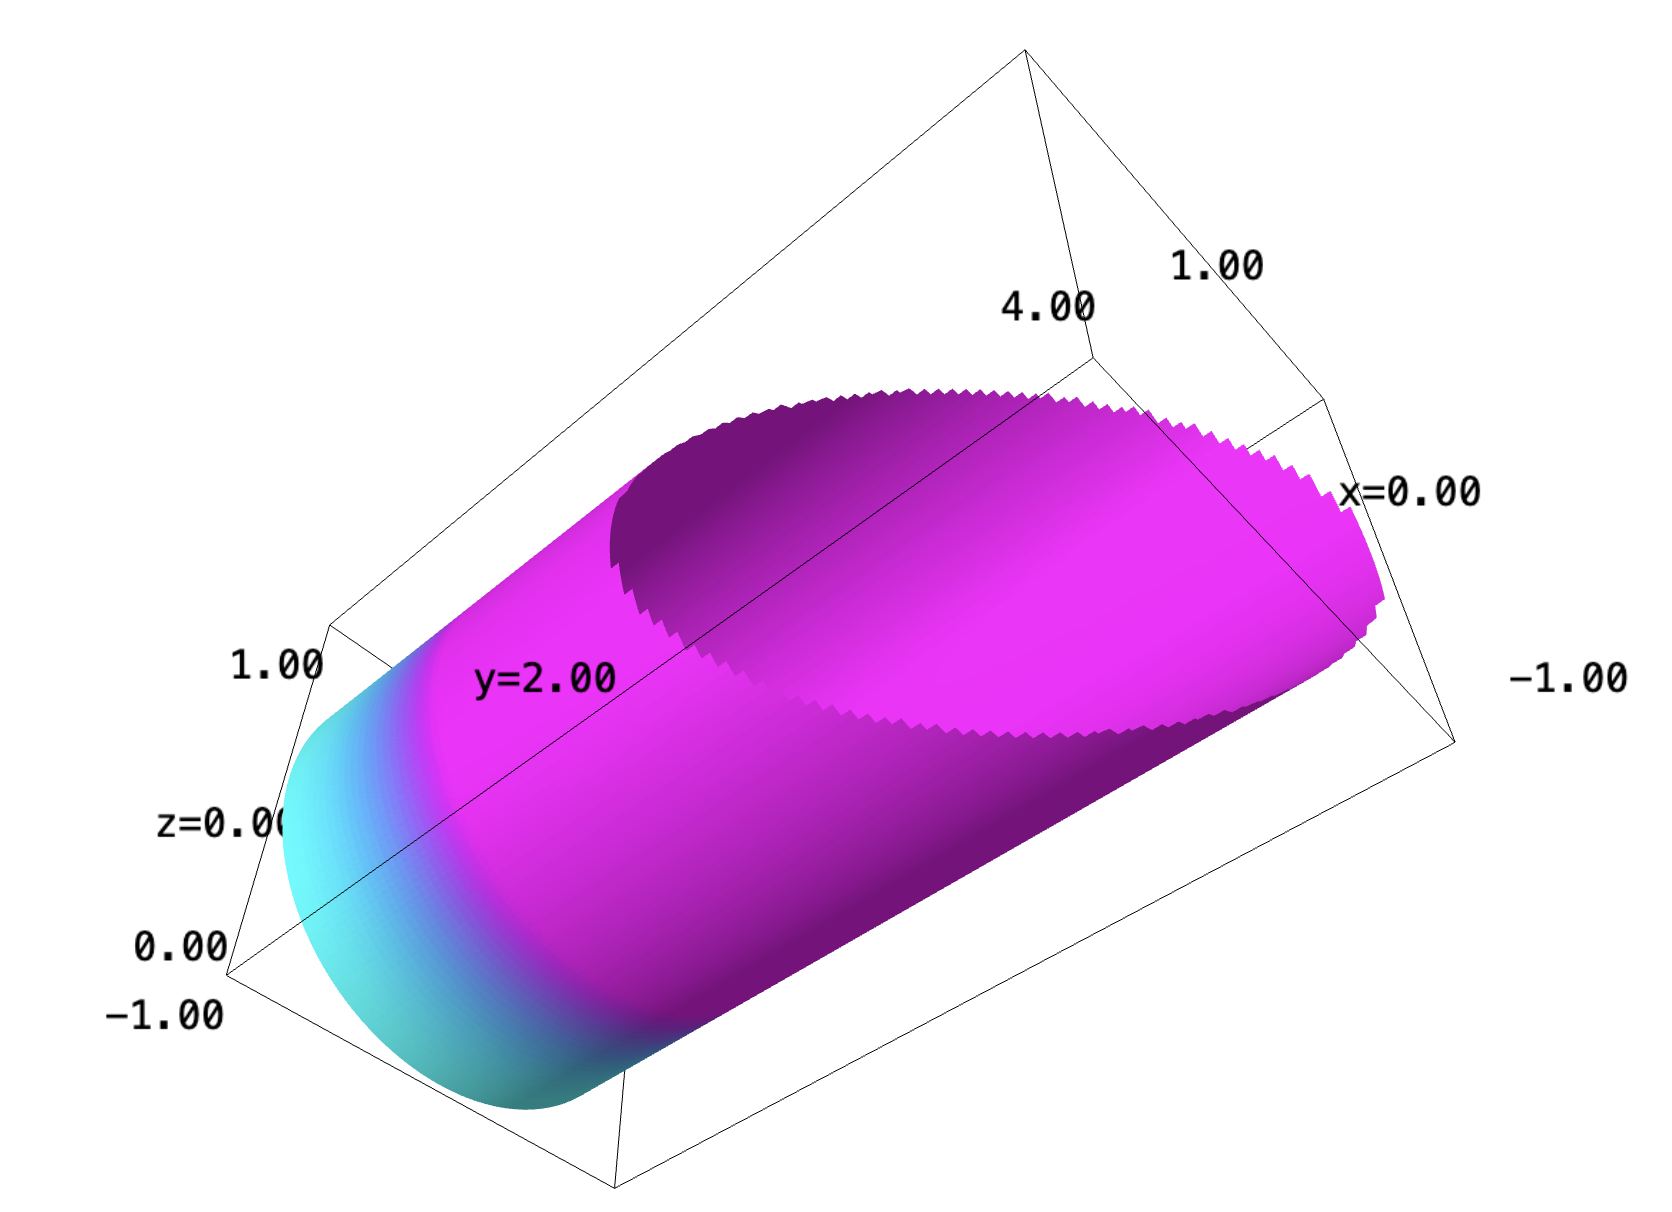
\includegraphics[width=.9\linewidth]{2022-05-23_10-16-40_screenshot.png}
\end{center}

that's honestly pretty cool!

Great, now let's take the actual surface integral. Note that, because the "pipe" does not have a defining ending point, we will set its end at the \(xy\) plane, that it ends at \(x=0\) at the other end in addition to \(y=3-x\).

Looking at the actual function for which we are taking the integral, we have:

\begin{equation}
   x^2 + z^2 = 1 
\end{equation}

We will rearrange this expression in terms of \(z\):

\begin{equation}
   z = \sqrt{1-x^2}
\end{equation}

Fortunately, we see already that the function's derivative w.r.t. \(y\) is \(0\); indeed, it doesn't change along the \(y\) direction (the cylinder is centered around it after all.)

Taking the derivative in the \(x\) direction:

\begin{align}
   \frac{\partial z}{\partial x} &= \frac{\partial}{\partial x} \sqrt{1-x^2} \\
&= \frac{-2x}{2\sqrt{-x^2+1}}\\
&= \frac{-x}{\sqrt{-x^2+1}}
\end{align}

Squaring the expression below:

\begin{equation}
\frac{x^2}{-x^2+1}
\end{equation}

And finally, we have the correction factor:

\begin{align}
    dA &= \sqrt{\frac{x^2}{-x^2+1} + 1}\ dV\\
&= \sqrt{\frac{1}{-x^2+1}}\ dV
\end{align}

Lastly, we can multiply the actual value function to this to this expression to get the expression for the integral:

\begin{equation}
   \iint_V\ y^2\ \sqrt{\frac{1}{-x^2+1}}\ dx\ dy
\end{equation}

Furthermore, our bounds are also a little complicated:

\begin{equation}
   \int_{-1}^1 \int_0^{3-x} \ y^2\ \sqrt{\frac{1}{-x^2+1}}\ dy\ dx
\end{equation}

Great, we will now ask Sage to take the actual integral for us:

\begin{verbatim}
f(x,y) = y^2*sqrt(1/(-x^2+1))
f.integrate(y, 0, 3-x).integrate(x, -1,1)
\end{verbatim}

\begin{verbatim}
21/2*pi
\end{verbatim}


Evidently, our result shows that the shape has a surface integral value of \(\frac{21\pi}{2} \approx 33\).

\section{Jacobian Matrix}
\label{sec:org32e8226}
We will attempt to take the derivative matrix for this expression methodically.

Let's define the function as:

\begin{equation}
   f(x,y,z) = (z^2-\sin(y)) \hat{h} + (x+y+z) \hat{i} + (e^y +7x) \hat{j} + (ln(x+y-2z)) \hat{k}
\end{equation}

\subsection{\(f_x\)}
\label{sec:org1dfd928}
\begin{itemize}
\item \(f_x \cdot {\hat{h}} = 0\)
\item \(f_x \cdot {\hat{i}} = 1\)
\item \(f_x \cdot {\hat{j}} = 7\)
\item \(f_x \cdot {\hat{k}} = \frac{1}{x+y-2z}\)
\end{itemize}

\subsection{\(f_y\)}
\label{sec:orgd60c2b4}
\begin{itemize}
\item \(f_y \cdot {\hat{h}} = -cos(y)\)
\item \(f_y \cdot {\hat{i}} = 1\)
\item \(f_y \cdot {\hat{j}} = e^y\)
\item \(f_y \cdot {\hat{k}} = \frac{1}{x+y-2z}\)
\end{itemize}

\subsection{\(f_z\)}
\label{sec:org0be4cd8}
\begin{itemize}
\item \(f_z \cdot {\hat{h}} = 0\)
\item \(f_z \cdot {\hat{i}} = 1\)
\item \(f_z \cdot {\hat{j}} = 0\)
\item \(f_z \cdot {\hat{k}} = \frac{-2}{x+y-2z}\)
\end{itemize}

\subsection{Jacobian}
\label{sec:org6c6f6e9}
Finally, we can assemble the Jacobian matrix

\begin{equation}
   \nabla f = \begin{bmatrix} 
0 & -\cos(y) & 0  \\
1 & 1 & 1 \\
7 & e^y & 0 \\
\frac{1}{x+y-2z} & \frac{1}{x+y-2z} & \frac{-2}{x+y-2z}
   \end{bmatrix} 
\end{equation}
\end{document}